\documentclass[twoside]{book}

% Packages required by doxygen
\usepackage{fixltx2e}
\usepackage{calc}
\usepackage{doxygen}
\usepackage[export]{adjustbox} % also loads graphicx
\usepackage{graphicx}
\usepackage[utf8]{inputenc}
\usepackage{makeidx}
\usepackage{multicol}
\usepackage{multirow}
\PassOptionsToPackage{warn}{textcomp}
\usepackage{textcomp}
\usepackage[nointegrals]{wasysym}
\usepackage[table]{xcolor}

% Font selection
\usepackage[T1]{fontenc}
\usepackage[scaled=.90]{helvet}
\usepackage{courier}
\usepackage{amssymb}
\usepackage{sectsty}
\renewcommand{\familydefault}{\sfdefault}
\allsectionsfont{%
  \fontseries{bc}\selectfont%
  \color{darkgray}%
}
\renewcommand{\DoxyLabelFont}{%
  \fontseries{bc}\selectfont%
  \color{darkgray}%
}
\newcommand{\+}{\discretionary{\mbox{\scriptsize$\hookleftarrow$}}{}{}}

% Page & text layout
\usepackage{geometry}
\geometry{%
  a4paper,%
  top=2.5cm,%
  bottom=2.5cm,%
  left=2.5cm,%
  right=2.5cm%
}
\tolerance=750
\hfuzz=15pt
\hbadness=750
\setlength{\emergencystretch}{15pt}
\setlength{\parindent}{0cm}
\setlength{\parskip}{3ex plus 2ex minus 2ex}
\makeatletter
\renewcommand{\paragraph}{%
  \@startsection{paragraph}{4}{0ex}{-1.0ex}{1.0ex}{%
    \normalfont\normalsize\bfseries\SS@parafont%
  }%
}
\renewcommand{\subparagraph}{%
  \@startsection{subparagraph}{5}{0ex}{-1.0ex}{1.0ex}{%
    \normalfont\normalsize\bfseries\SS@subparafont%
  }%
}
\makeatother

% Headers & footers
\usepackage{fancyhdr}
\pagestyle{fancyplain}
\fancyhead[LE]{\fancyplain{}{\bfseries\thepage}}
\fancyhead[CE]{\fancyplain{}{}}
\fancyhead[RE]{\fancyplain{}{\bfseries\leftmark}}
\fancyhead[LO]{\fancyplain{}{\bfseries\rightmark}}
\fancyhead[CO]{\fancyplain{}{}}
\fancyhead[RO]{\fancyplain{}{\bfseries\thepage}}
\fancyfoot[LE]{\fancyplain{}{}}
\fancyfoot[CE]{\fancyplain{}{}}
\fancyfoot[RE]{\fancyplain{}{\bfseries\scriptsize Generated by Doxygen }}
\fancyfoot[LO]{\fancyplain{}{\bfseries\scriptsize Generated by Doxygen }}
\fancyfoot[CO]{\fancyplain{}{}}
\fancyfoot[RO]{\fancyplain{}{}}
\renewcommand{\footrulewidth}{0.4pt}
\renewcommand{\chaptermark}[1]{%
  \markboth{#1}{}%
}
\renewcommand{\sectionmark}[1]{%
  \markright{\thesection\ #1}%
}

% Indices & bibliography
\usepackage{natbib}
\usepackage[titles]{tocloft}
\setcounter{tocdepth}{3}
\setcounter{secnumdepth}{5}
\makeindex

% Hyperlinks (required, but should be loaded last)
\usepackage{ifpdf}
\ifpdf
  \usepackage[pdftex,pagebackref=true]{hyperref}
\else
  \usepackage[ps2pdf,pagebackref=true]{hyperref}
\fi
\hypersetup{%
  colorlinks=true,%
  linkcolor=blue,%
  citecolor=blue,%
  unicode%
}

% Custom commands
\newcommand{\clearemptydoublepage}{%
  \newpage{\pagestyle{empty}\cleardoublepage}%
}

\usepackage{caption}
\captionsetup{labelsep=space,justification=centering,font={bf},singlelinecheck=off,skip=4pt,position=top}

%===== C O N T E N T S =====

\begin{document}

% Titlepage & ToC
\hypersetup{pageanchor=false,
             bookmarksnumbered=true,
             pdfencoding=unicode
            }
\pagenumbering{roman}
\begin{titlepage}
\vspace*{7cm}
\begin{center}%
{\Large My Project }\\
\vspace*{1cm}
{\large Generated by Doxygen 1.8.11}\\
\end{center}
\end{titlepage}
\clearemptydoublepage
\tableofcontents
\clearemptydoublepage
\pagenumbering{arabic}
\hypersetup{pageanchor=true}

%--- Begin generated contents ---
\chapter{R\+E\+A\+D\+ME}
\label{md_README}
\hypertarget{md_README}{}
Här ligger andra lageruppgiften 
\chapter{Class Index}
\section{Class List}
Here are the classes, structs, unions and interfaces with brief descriptions\+:\begin{DoxyCompactList}
\item\contentsline{section}{\hyperlink{unionanswer__t}{answer\+\_\+t} }{\pageref{unionanswer__t}}{}
\item\contentsline{section}{\hyperlink{structelem__array}{elem\+\_\+array} }{\pageref{structelem__array}}{}
\item\contentsline{section}{\hyperlink{unionelement}{element} }{\pageref{unionelement}}{}
\item\contentsline{section}{\hyperlink{structitem}{item} }{\pageref{structitem}}{}
\item\contentsline{section}{\hyperlink{structlink}{link} }{\pageref{structlink}}{}
\item\contentsline{section}{\hyperlink{structlist}{list} }{\pageref{structlist}}{}
\item\contentsline{section}{\hyperlink{structnode}{node} }{\pageref{structnode}}{}
\item\contentsline{section}{\hyperlink{structshelf}{shelf} }{\pageref{structshelf}}{}
\item\contentsline{section}{\hyperlink{structtest}{test} }{\pageref{structtest}}{}
\item\contentsline{section}{\hyperlink{structtree}{tree} }{\pageref{structtree}}{}
\end{DoxyCompactList}

\chapter{Class Documentation}
\hypertarget{unionanswer__t}{}\section{answer\+\_\+t unionreferens}
\label{unionanswer__t}\index{answer\+\_\+t@{answer\+\_\+t}}
\subsection*{Datafält}
\begin{DoxyCompactItemize}
\item 
int \hyperlink{unionanswer__t_a21d3d2b485a0dcf04e6ec6a60bb4d4db}{i}
\item 
float \hyperlink{unionanswer__t_acc96d348401060d8beea19445f9fe184}{f}
\item 
char $\ast$ \hyperlink{unionanswer__t_a0de66e8519f97035ac10688155603648}{s}
\item 
char \hyperlink{unionanswer__t_af43a34a48344362715fc22573522dbfa}{c}
\end{DoxyCompactItemize}


\subsection{Fält dokumentation}
\index{answer\+\_\+t@{answer\+\_\+t}!c@{c}}
\index{c@{c}!answer\+\_\+t@{answer\+\_\+t}}
\subsubsection[{\texorpdfstring{c}{c}}]{\setlength{\rightskip}{0pt plus 5cm}char answer\+\_\+t\+::c}\hypertarget{unionanswer__t_af43a34a48344362715fc22573522dbfa}{}\label{unionanswer__t_af43a34a48344362715fc22573522dbfa}
\index{answer\+\_\+t@{answer\+\_\+t}!f@{f}}
\index{f@{f}!answer\+\_\+t@{answer\+\_\+t}}
\subsubsection[{\texorpdfstring{f}{f}}]{\setlength{\rightskip}{0pt plus 5cm}float answer\+\_\+t\+::f}\hypertarget{unionanswer__t_acc96d348401060d8beea19445f9fe184}{}\label{unionanswer__t_acc96d348401060d8beea19445f9fe184}
\index{answer\+\_\+t@{answer\+\_\+t}!i@{i}}
\index{i@{i}!answer\+\_\+t@{answer\+\_\+t}}
\subsubsection[{\texorpdfstring{i}{i}}]{\setlength{\rightskip}{0pt plus 5cm}int answer\+\_\+t\+::i}\hypertarget{unionanswer__t_a21d3d2b485a0dcf04e6ec6a60bb4d4db}{}\label{unionanswer__t_a21d3d2b485a0dcf04e6ec6a60bb4d4db}
\index{answer\+\_\+t@{answer\+\_\+t}!s@{s}}
\index{s@{s}!answer\+\_\+t@{answer\+\_\+t}}
\subsubsection[{\texorpdfstring{s}{s}}]{\setlength{\rightskip}{0pt plus 5cm}char$\ast$ answer\+\_\+t\+::s}\hypertarget{unionanswer__t_a0de66e8519f97035ac10688155603648}{}\label{unionanswer__t_a0de66e8519f97035ac10688155603648}


Dokumentationen för denna union var genererad från följande fil\+:\begin{DoxyCompactItemize}
\item 
\hyperlink{utils_8c}{utils.\+c}\end{DoxyCompactItemize}

\hypertarget{structelem__array}{}\section{elem\+\_\+array Struct Reference}
\label{structelem__array}\index{elem\+\_\+array@{elem\+\_\+array}}


Collaboration diagram for elem\+\_\+array\+:

\hypertarget{unionelement}{}\section{element unionreferens}
\label{unionelement}\index{element@{element}}


{\ttfamily \#include $<$common.\+h$>$}

\subsection*{Datafält}
\begin{DoxyCompactItemize}
\item 
int \hyperlink{unionelement_a4e41a1440036146f7a3c50c07a91e7fe}{i}
\item 
uint \hyperlink{unionelement_abd4034f37eb6d6ecdda71c9102680902}{u}
\item 
void $\ast$ \hyperlink{unionelement_a075c65aee9ffc316eb213e9d0606e0b9}{p}
\item 
float \hyperlink{unionelement_a8cf2d86c582a0e86d5f1ee1e4f62816b}{f}
\end{DoxyCompactItemize}


\subsection{Detaljerad beskrivning}
Element wrapper

Elements in the list are stored inside an elem\+\_\+t which is passed in by copy. 

\subsection{Fält dokumentation}
\index{element@{element}!f@{f}}
\index{f@{f}!element@{element}}
\subsubsection[{\texorpdfstring{f}{f}}]{\setlength{\rightskip}{0pt plus 5cm}float element\+::f}\hypertarget{unionelement_a8cf2d86c582a0e86d5f1ee1e4f62816b}{}\label{unionelement_a8cf2d86c582a0e86d5f1ee1e4f62816b}
\index{element@{element}!i@{i}}
\index{i@{i}!element@{element}}
\subsubsection[{\texorpdfstring{i}{i}}]{\setlength{\rightskip}{0pt plus 5cm}int element\+::i}\hypertarget{unionelement_a4e41a1440036146f7a3c50c07a91e7fe}{}\label{unionelement_a4e41a1440036146f7a3c50c07a91e7fe}
\index{element@{element}!p@{p}}
\index{p@{p}!element@{element}}
\subsubsection[{\texorpdfstring{p}{p}}]{\setlength{\rightskip}{0pt plus 5cm}void$\ast$ element\+::p}\hypertarget{unionelement_a075c65aee9ffc316eb213e9d0606e0b9}{}\label{unionelement_a075c65aee9ffc316eb213e9d0606e0b9}
\index{element@{element}!u@{u}}
\index{u@{u}!element@{element}}
\subsubsection[{\texorpdfstring{u}{u}}]{\setlength{\rightskip}{0pt plus 5cm}uint element\+::u}\hypertarget{unionelement_abd4034f37eb6d6ecdda71c9102680902}{}\label{unionelement_abd4034f37eb6d6ecdda71c9102680902}


Dokumentationen för denna union var genererad från följande fil\+:\begin{DoxyCompactItemize}
\item 
\hyperlink{common_8h}{common.\+h}\end{DoxyCompactItemize}

\hypertarget{structitem}{}\section{item struktreferens}
\label{structitem}\index{item@{item}}


Samarbetsdiagram för item\+:\nopagebreak
\begin{figure}[H]
\begin{center}
\leavevmode
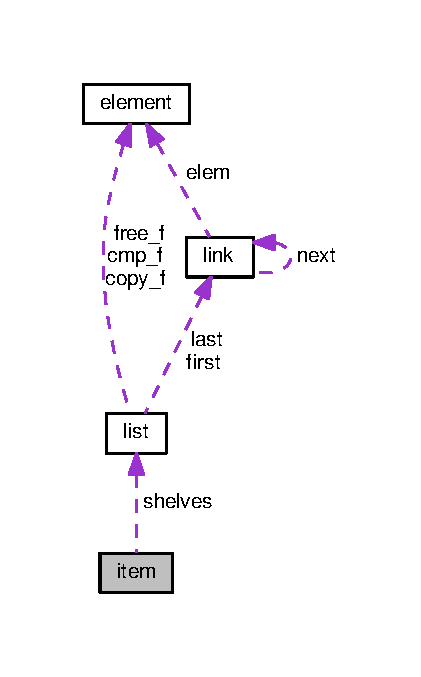
\includegraphics[width=202pt]{structitem__coll__graph}
\end{center}
\end{figure}
\subsection*{Datafält}
\begin{DoxyCompactItemize}
\item 
char $\ast$ \hyperlink{structitem_adbf6cb817816601a08c614bb77bcf075}{name}
\item 
char $\ast$ \hyperlink{structitem_a7486c43d6e783fd7093dc9cee62b518f}{descr}
\item 
int \hyperlink{structitem_a77214da8535815143a7ba318a25c5811}{price}
\item 
\hyperlink{list_8h_a15376354e4e8b4f1732e9df17f30786c}{list\+\_\+t} $\ast$ \hyperlink{structitem_a2c6c18e4202d967e7ff0f4421b72bcdf}{shelves}
\end{DoxyCompactItemize}


\subsection{Fält dokumentation}
\index{item@{item}!descr@{descr}}
\index{descr@{descr}!item@{item}}
\subsubsection[{\texorpdfstring{descr}{descr}}]{\setlength{\rightskip}{0pt plus 5cm}char$\ast$ item\+::descr}\hypertarget{structitem_a7486c43d6e783fd7093dc9cee62b518f}{}\label{structitem_a7486c43d6e783fd7093dc9cee62b518f}
Varans beskrivning \index{item@{item}!name@{name}}
\index{name@{name}!item@{item}}
\subsubsection[{\texorpdfstring{name}{name}}]{\setlength{\rightskip}{0pt plus 5cm}char$\ast$ item\+::name}\hypertarget{structitem_adbf6cb817816601a08c614bb77bcf075}{}\label{structitem_adbf6cb817816601a08c614bb77bcf075}
Varans namn i form av en textsträng \index{item@{item}!price@{price}}
\index{price@{price}!item@{item}}
\subsubsection[{\texorpdfstring{price}{price}}]{\setlength{\rightskip}{0pt plus 5cm}int item\+::price}\hypertarget{structitem_a77214da8535815143a7ba318a25c5811}{}\label{structitem_a77214da8535815143a7ba318a25c5811}
Varans pris \index{item@{item}!shelves@{shelves}}
\index{shelves@{shelves}!item@{item}}
\subsubsection[{\texorpdfstring{shelves}{shelves}}]{\setlength{\rightskip}{0pt plus 5cm}{\bf list\+\_\+t}$\ast$ item\+::shelves}\hypertarget{structitem_a2c6c18e4202d967e7ff0f4421b72bcdf}{}\label{structitem_a2c6c18e4202d967e7ff0f4421b72bcdf}
\hyperlink{structEn}{En} lista av varuhyllor 

Dokumentationen för denna strukt var genererad från följande fil\+:\begin{DoxyCompactItemize}
\item 
\hyperlink{item_8c}{item.\+c}\end{DoxyCompactItemize}

\hypertarget{structlink}{}\section{link struktreferens}
\label{structlink}\index{link@{link}}


Samarbetsdiagram för link\+:\nopagebreak
\begin{figure}[H]
\begin{center}
\leavevmode
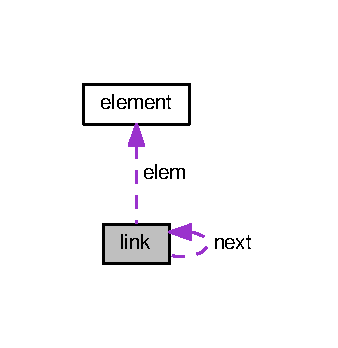
\includegraphics[width=162pt]{structlink__coll__graph}
\end{center}
\end{figure}
\subsection*{Datafält}
\begin{DoxyCompactItemize}
\item 
\hyperlink{common_8h_a7fdd31df4fac71b8c34af47c7d45226a}{elem\+\_\+t} \hyperlink{structlink_a83c7f47df8ba3635bf45c0b8debffde5}{elem}
\item 
\hyperlink{list_8c_ab1a5f2fcda4f00dce92c82ebc30c4b3d}{link\+\_\+t} $\ast$ \hyperlink{structlink_a5e51af3becfae77d89502036a8e508c2}{next}
\end{DoxyCompactItemize}


\subsection{Fält dokumentation}
\index{link@{link}!elem@{elem}}
\index{elem@{elem}!link@{link}}
\subsubsection[{\texorpdfstring{elem}{elem}}]{\setlength{\rightskip}{0pt plus 5cm}{\bf elem\+\_\+t} link\+::elem}\hypertarget{structlink_a83c7f47df8ba3635bf45c0b8debffde5}{}\label{structlink_a83c7f47df8ba3635bf45c0b8debffde5}
\index{link@{link}!next@{next}}
\index{next@{next}!link@{link}}
\subsubsection[{\texorpdfstring{next}{next}}]{\setlength{\rightskip}{0pt plus 5cm}{\bf link\+\_\+t}$\ast$ link\+::next}\hypertarget{structlink_a5e51af3becfae77d89502036a8e508c2}{}\label{structlink_a5e51af3becfae77d89502036a8e508c2}


Dokumentationen för denna strukt var genererad från följande fil\+:\begin{DoxyCompactItemize}
\item 
\hyperlink{list_8c}{list.\+c}\end{DoxyCompactItemize}

\hypertarget{structlist}{}\section{list Struct Reference}
\label{structlist}\index{list@{list}}


Collaboration diagram for list\+:
% FIG 0
\subsection*{Public Attributes}
\begin{DoxyCompactItemize}
\item 
\hyperlink{structlink}{link\+\_\+t} $\ast$ {\bfseries first}\hypertarget{structlist_a8b3138e762449dc038dfa560f02f5f96}{}\label{structlist_a8b3138e762449dc038dfa560f02f5f96}

\item 
\hyperlink{structlink}{link\+\_\+t} $\ast$ {\bfseries last}\hypertarget{structlist_a05a1dc6800f93b4e20b872a397ab396f}{}\label{structlist_a05a1dc6800f93b4e20b872a397ab396f}

\item 
element\+\_\+copy\+\_\+fun {\bfseries copy\+\_\+f}\hypertarget{structlist_acd5def2fe519248ad24e10b426acd44f}{}\label{structlist_acd5def2fe519248ad24e10b426acd44f}

\item 
element\+\_\+free\+\_\+fun {\bfseries free\+\_\+f}\hypertarget{structlist_a28ae85a352de920c1bcc353411bac5fe}{}\label{structlist_a28ae85a352de920c1bcc353411bac5fe}

\item 
element\+\_\+comp\+\_\+fun {\bfseries cmp\+\_\+f}\hypertarget{structlist_a3e595459af1efe57e5929c7a48c1cb1c}{}\label{structlist_a3e595459af1efe57e5929c7a48c1cb1c}

\item 
size\+\_\+t {\bfseries size}\hypertarget{structlist_ae581be90bd8eb7051528b61ad216de88}{}\label{structlist_ae581be90bd8eb7051528b61ad216de88}

\end{DoxyCompactItemize}


The documentation for this struct was generated from the following file\+:\begin{DoxyCompactItemize}
\item 
list.\+c\end{DoxyCompactItemize}

\hypertarget{structnode}{}\section{node struktreferens}
\label{structnode}\index{node@{node}}


Samarbetsdiagram för node\+:\nopagebreak
\begin{figure}[H]
\begin{center}
\leavevmode
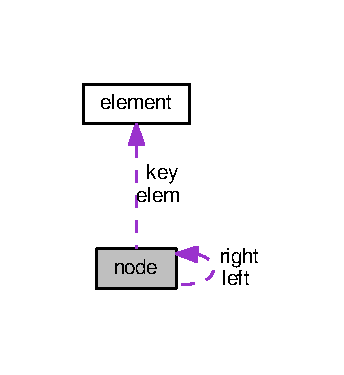
\includegraphics[width=165pt]{structnode__coll__graph}
\end{center}
\end{figure}
\subsection*{Datafält}
\begin{DoxyCompactItemize}
\item 
\hyperlink{common_8h_a7fdd31df4fac71b8c34af47c7d45226a}{elem\+\_\+t} \hyperlink{structnode_a5f9ee8710ff865cda6ed144d91a32121}{elem}
\item 
\hyperlink{tree_8h_af42dd67b55ffc67649d20c46e9cbf84f}{tree\+\_\+key\+\_\+t} \hyperlink{structnode_aa6b692707ee43532d0437efb6f060dfd}{key}
\item 
\hyperlink{tree_8h_a7c02633e18d6aa5f58539b75f08753d9}{node\+\_\+t} $\ast$ \hyperlink{structnode_aacd557e63e1f9dca9048ed58bb3dbb2c}{left}
\item 
\hyperlink{tree_8h_a7c02633e18d6aa5f58539b75f08753d9}{node\+\_\+t} $\ast$ \hyperlink{structnode_a8ab67b704953f3699d566a1a5d6047ad}{right}
\end{DoxyCompactItemize}


\subsection{Fält dokumentation}
\index{node@{node}!elem@{elem}}
\index{elem@{elem}!node@{node}}
\subsubsection[{\texorpdfstring{elem}{elem}}]{\setlength{\rightskip}{0pt plus 5cm}{\bf elem\+\_\+t} node\+::elem}\hypertarget{structnode_a5f9ee8710ff865cda6ed144d91a32121}{}\label{structnode_a5f9ee8710ff865cda6ed144d91a32121}
\index{node@{node}!key@{key}}
\index{key@{key}!node@{node}}
\subsubsection[{\texorpdfstring{key}{key}}]{\setlength{\rightskip}{0pt plus 5cm}{\bf tree\+\_\+key\+\_\+t} node\+::key}\hypertarget{structnode_aa6b692707ee43532d0437efb6f060dfd}{}\label{structnode_aa6b692707ee43532d0437efb6f060dfd}
\index{node@{node}!left@{left}}
\index{left@{left}!node@{node}}
\subsubsection[{\texorpdfstring{left}{left}}]{\setlength{\rightskip}{0pt plus 5cm}{\bf node\+\_\+t}$\ast$ node\+::left}\hypertarget{structnode_aacd557e63e1f9dca9048ed58bb3dbb2c}{}\label{structnode_aacd557e63e1f9dca9048ed58bb3dbb2c}
\index{node@{node}!right@{right}}
\index{right@{right}!node@{node}}
\subsubsection[{\texorpdfstring{right}{right}}]{\setlength{\rightskip}{0pt plus 5cm}{\bf node\+\_\+t}$\ast$ node\+::right}\hypertarget{structnode_a8ab67b704953f3699d566a1a5d6047ad}{}\label{structnode_a8ab67b704953f3699d566a1a5d6047ad}


Dokumentationen för denna strukt var genererad från följande fil\+:\begin{DoxyCompactItemize}
\item 
\hyperlink{tree_8c}{tree.\+c}\end{DoxyCompactItemize}

\hypertarget{structshelf}{}\section{shelf struktreferens}
\label{structshelf}\index{shelf@{shelf}}
\subsection*{Datafält}
\begin{DoxyCompactItemize}
\item 
char $\ast$ \hyperlink{structshelf_a7f8287189403254107701949e95c307a}{id}
\item 
int \hyperlink{structshelf_a6a1b09835f421eb1aa0d752411484733}{amount}
\end{DoxyCompactItemize}


\subsection{Fält dokumentation}
\index{shelf@{shelf}!amount@{amount}}
\index{amount@{amount}!shelf@{shelf}}
\subsubsection[{\texorpdfstring{amount}{amount}}]{\setlength{\rightskip}{0pt plus 5cm}int shelf\+::amount}\hypertarget{structshelf_a6a1b09835f421eb1aa0d752411484733}{}\label{structshelf_a6a1b09835f421eb1aa0d752411484733}
Antal varor lagrade på hyllan \index{shelf@{shelf}!id@{id}}
\index{id@{id}!shelf@{shelf}}
\subsubsection[{\texorpdfstring{id}{id}}]{\setlength{\rightskip}{0pt plus 5cm}char$\ast$ shelf\+::id}\hypertarget{structshelf_a7f8287189403254107701949e95c307a}{}\label{structshelf_a7f8287189403254107701949e95c307a}
Hyllans namn 

Dokumentationen för denna strukt var genererad från följande fil\+:\begin{DoxyCompactItemize}
\item 
\hyperlink{item_8c}{item.\+c}\end{DoxyCompactItemize}

\hypertarget{structtest}{}\section{test struktreferens}
\label{structtest}\index{test@{test}}
\subsection*{Datafält}
\begin{DoxyCompactItemize}
\item 
char $\ast$ \hyperlink{structtest_aad4bcf4a89644c9ad3adc507df7eef15}{a}
\item 
int \hyperlink{structtest_ac52450ad7e71deba8e07a10cfea034ed}{b}
\end{DoxyCompactItemize}


\subsection{Fält dokumentation}
\index{test@{test}!a@{a}}
\index{a@{a}!test@{test}}
\subsubsection[{\texorpdfstring{a}{a}}]{\setlength{\rightskip}{0pt plus 5cm}char$\ast$ test\+::a}\hypertarget{structtest_aad4bcf4a89644c9ad3adc507df7eef15}{}\label{structtest_aad4bcf4a89644c9ad3adc507df7eef15}
\index{test@{test}!b@{b}}
\index{b@{b}!test@{test}}
\subsubsection[{\texorpdfstring{b}{b}}]{\setlength{\rightskip}{0pt plus 5cm}int test\+::b}\hypertarget{structtest_ac52450ad7e71deba8e07a10cfea034ed}{}\label{structtest_ac52450ad7e71deba8e07a10cfea034ed}


Dokumentationen för denna strukt var genererad från följande fil\+:\begin{DoxyCompactItemize}
\item 
\hyperlink{lager_8c}{lager.\+c}\end{DoxyCompactItemize}

\hypertarget{structtree}{}\section{tree Struct Reference}
\label{structtree}\index{tree@{tree}}


Collaboration diagram for tree\+:
% FIG 0
\subsection*{Public Attributes}
\begin{DoxyCompactItemize}
\item 
\hyperlink{structnode}{node\+\_\+t} $\ast$ {\bfseries root}\hypertarget{structtree_a1c9d515ea8291ba3e8dd27a32ad11c99}{}\label{structtree_a1c9d515ea8291ba3e8dd27a32ad11c99}

\item 
element\+\_\+copy\+\_\+fun {\bfseries copy\+\_\+f}\hypertarget{structtree_a612e416ae22a51e05773a4ed5a673a95}{}\label{structtree_a612e416ae22a51e05773a4ed5a673a95}

\item 
element\+\_\+free\+\_\+fun {\bfseries e\+\_\+free\+\_\+f}\hypertarget{structtree_a52ca9019231724325da51c920ba98b83}{}\label{structtree_a52ca9019231724325da51c920ba98b83}

\item 
key\+\_\+free\+\_\+fun {\bfseries k\+\_\+free\+\_\+f}\hypertarget{structtree_a2a6ff28f2b42cea10f416f6e0fd4f540}{}\label{structtree_a2a6ff28f2b42cea10f416f6e0fd4f540}

\item 
element\+\_\+comp\+\_\+fun {\bfseries cmp\+\_\+f}\hypertarget{structtree_a4bbea9002bc047957acc4672113cac7c}{}\label{structtree_a4bbea9002bc047957acc4672113cac7c}

\item 
size\+\_\+t {\bfseries size}\hypertarget{structtree_a794fa86f6b2815f255a79b3a46fdb190}{}\label{structtree_a794fa86f6b2815f255a79b3a46fdb190}

\end{DoxyCompactItemize}


The documentation for this struct was generated from the following file\+:\begin{DoxyCompactItemize}
\item 
tree.\+c\end{DoxyCompactItemize}

%--- End generated contents ---

% Index
\backmatter
\newpage
\phantomsection
\clearemptydoublepage
\addcontentsline{toc}{chapter}{Index}
\printindex

\end{document}
